\documentclass[12pt]{article}

\usepackage{setspace}
\usepackage{caption}
\usepackage{subcaption}
\usepackage{float}
\usepackage{makecell}
\usepackage{amsmath}
\usepackage{graphicx}
\graphicspath{ {./images/} }
\usepackage[utf8]{inputenc}
\usepackage[russian]{babel}
\usepackage{geometry}
 \geometry{
 a4paper,
 left=20mm,
 right=20mm,
 top=20mm,
 bot=20mm,
 }

\begin{document}

\begin{titlepage}
\begin{center}
    НАЦИОНАЛЬНЫЙ ИССЛЕДОВАТЕЛЬСКИЙ УНИВЕРСИТЕТ ИТМО \\
    Факультет систем управления и робототехники \\
    \vspace*{10\baselineskip}
    {\LARGEЭлектротехника} \\
    \ \\
    \ \\
    \begin{spacing}{1.5}
    {\large Лабораторная работа №2 \\
    ИССЛЕДОВАНИЕ ЛИНЕЙНЫХ ДВУХПОЛЮСНИКОВ \\
    \ \\
    Вариант 3R382}
    \end{spacing} \\
    \ \\
    \vspace*{10\baselineskip}
    \hfill {Студент: Кирбаба Д.Д.\ \ \ \ \ \ \ \ \ } \\
    \hfill {Группа: R3338\ \ \ \ \ \ \ \ \ \ \ \ \ \ \ \ \ \ \ \ \ } \\
    \hfill {Преподаватель: Китаев Ю.В.} \\
    \mbox{}
    \vfill {г. Санкт-Петербург\\2023}
\end{center}
\end{titlepage}

\subsubsection*{Цель работы}
Исследование режимов работы и экспериментальное определение параметров линейной схемы, подключенной к источнику питания синусоидального тока.

\subsubsection*{Ход работы}
\begin{figure}[H]
    \centering
    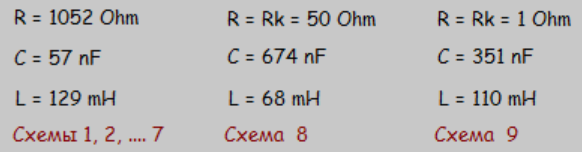
\includegraphics[width=0.7\textwidth]{initial_data.png}
    \caption{Начальные данные.}
    \label{fig:initial_data}
\end{figure}

Проведем моделирование для 7 различных типов двухполюсников, используя данный шаблон:

\begin{figure}[H]
    \centering
    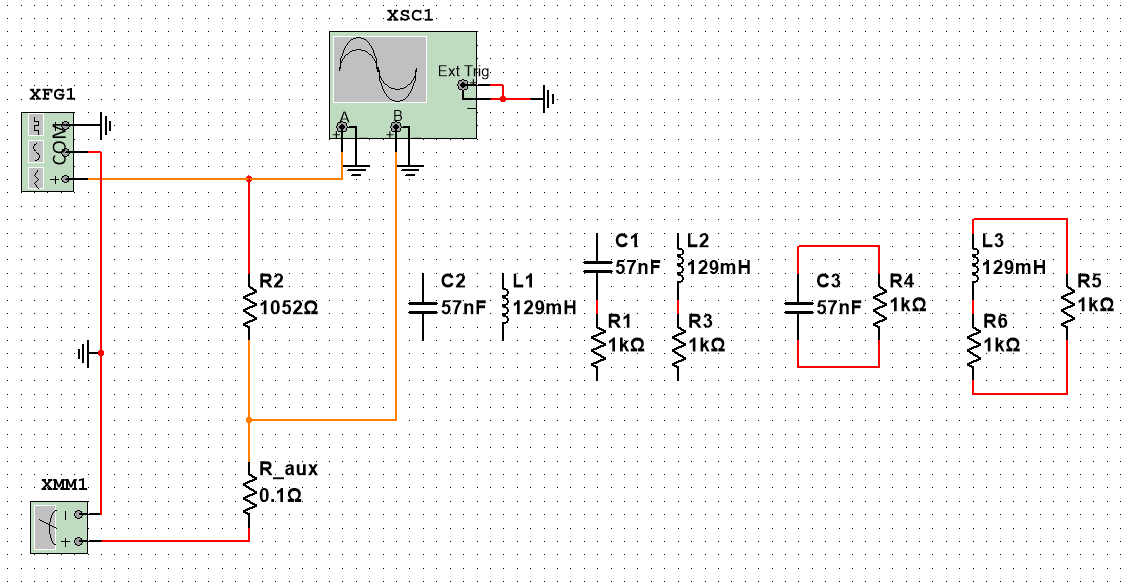
\includegraphics[width=0.7\textwidth]{scheme.png}
    \caption{Схема моделирования для первых 7 типов.}
    \label{fig:scheme}
\end{figure}

\begin{figure}[H]
    \centering
    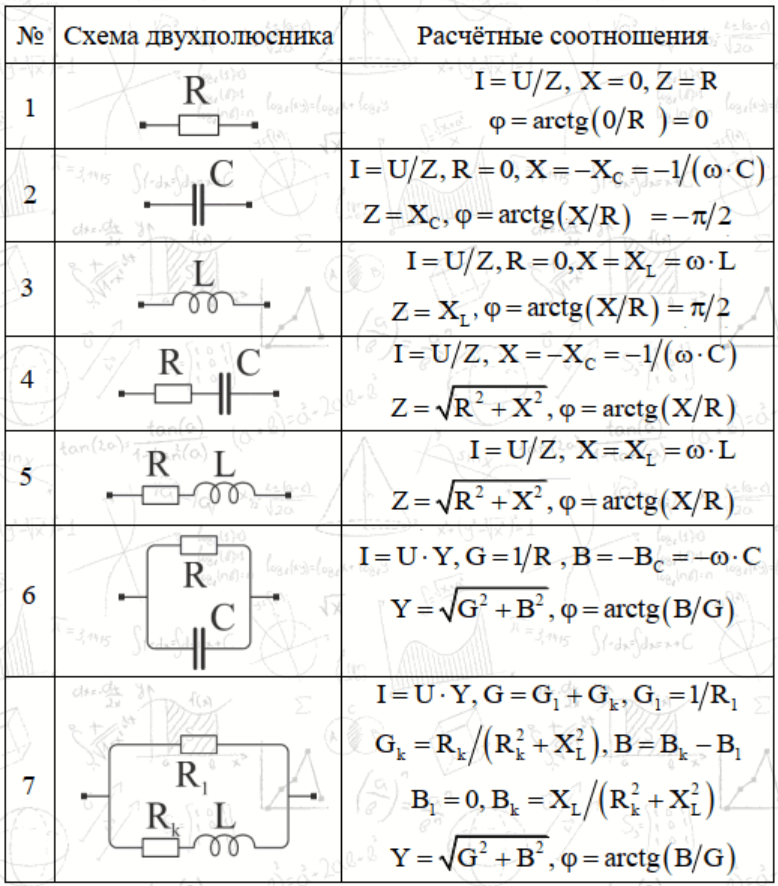
\includegraphics[width=0.5\textwidth]{table.png}
    \caption{Двухполюсники и расчетные формулы.}
    \label{fig:table}
\end{figure}

Заполним таблицу результатами измерений, вычислений и параметров двухполюсников:
\begin{figure}[H]
    \centering
    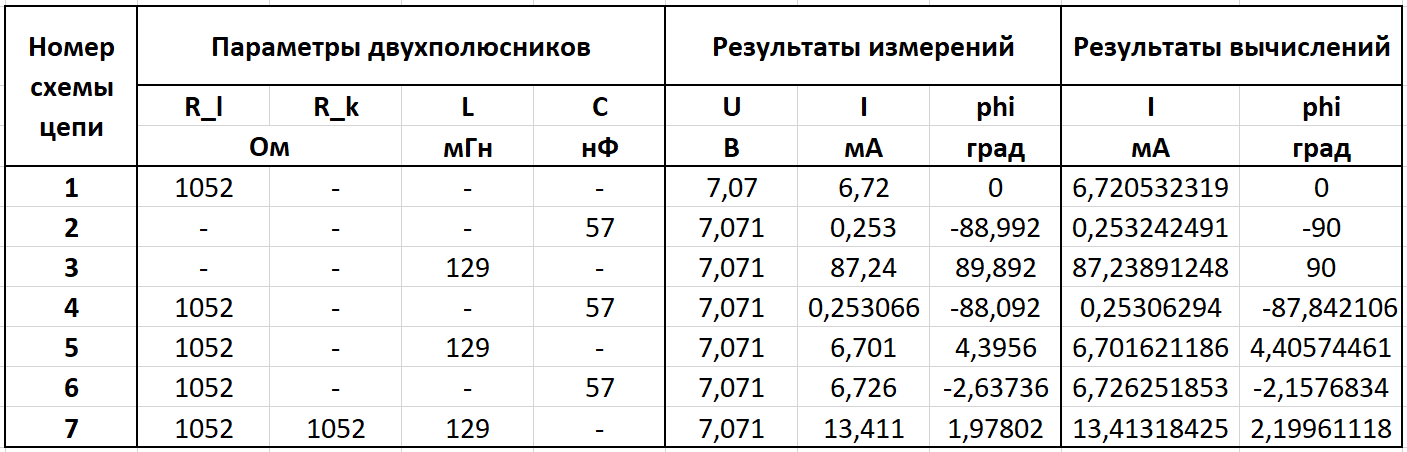
\includegraphics[width=\textwidth]{table_1_7.png}
    \caption{Расчетная таблица для первых 7 типов двухполюсников.}
    \label{fig:table_1_7}
\end{figure}

Для исследования последовательного резонанса, будем использовать следующую схему моделирования с последовательной RLC цепочкой:
\begin{figure}[H]
    \centering
    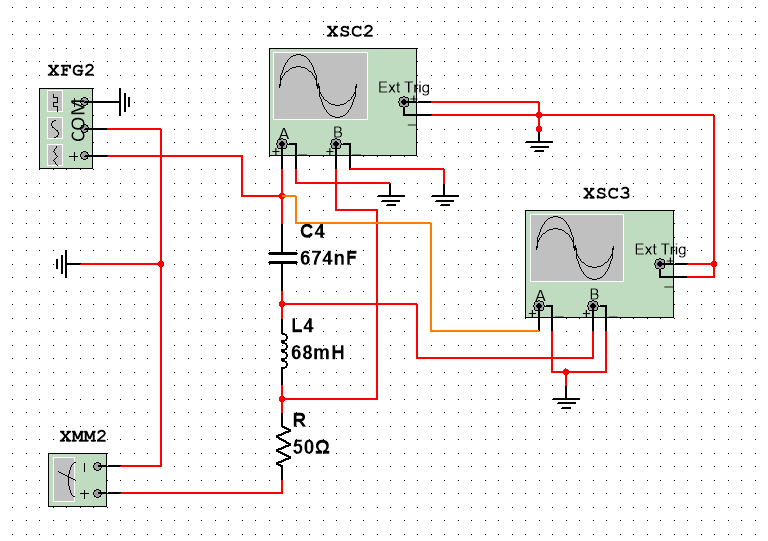
\includegraphics[width=0.7\textwidth]{8_scheme.png}
    \caption{Схема моделирования последовательного резонанса.}
    \label{fig:8_scheme}
\end{figure}

Рассчитаем резонансную частоту:
\[  
    f_0 = \frac{1}{2 \pi \sqrt(LC)} = 743 \ Hz
\]

Теперь установим вычисленную резонансную частоту на генераторе напряжения:
\begin{figure}[H]
    \centering
    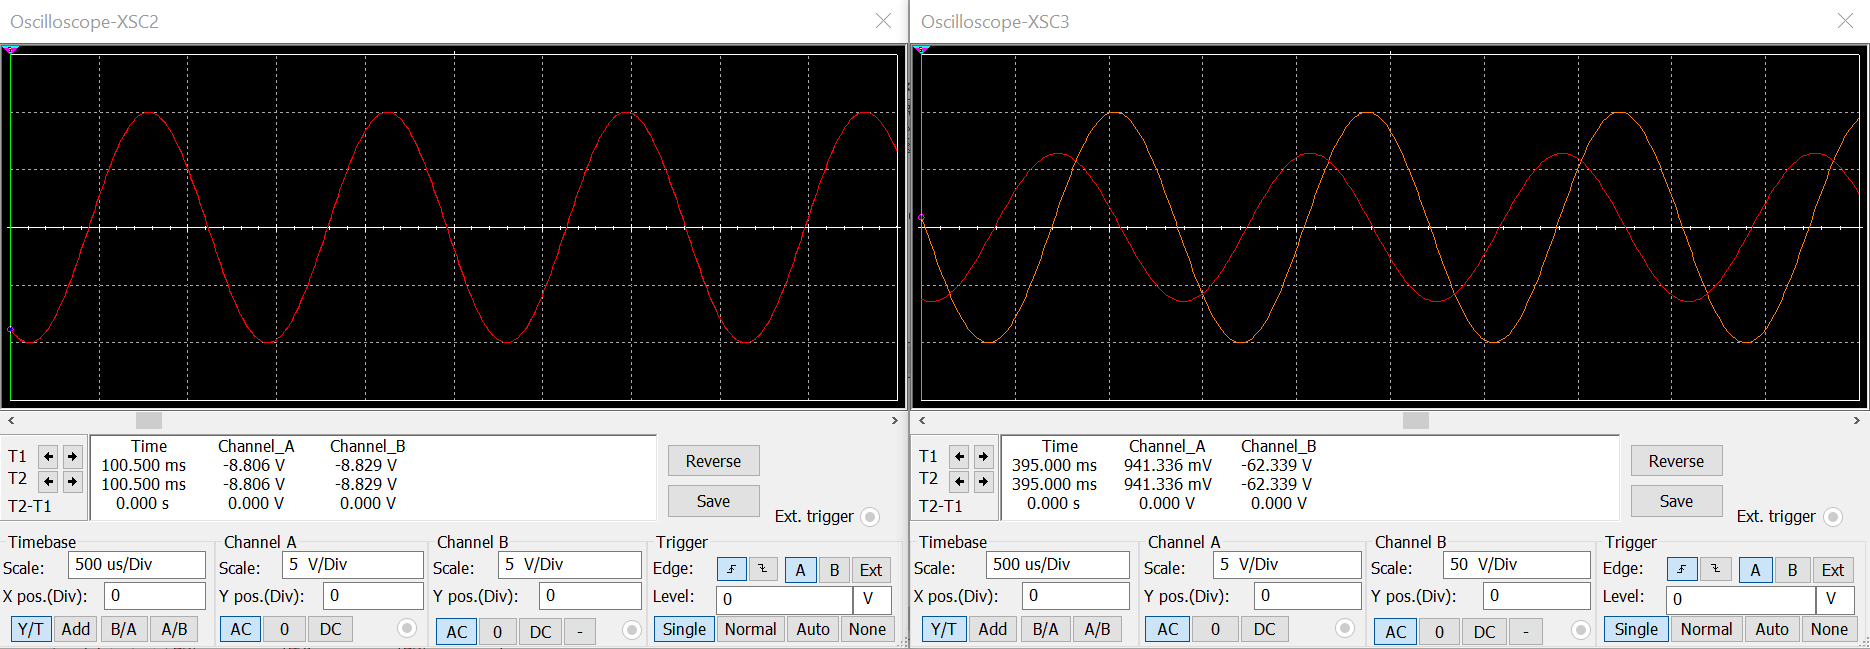
\includegraphics[width=\textwidth]{8_osc_plots.png}
    \caption{Осциллограммы при последовательном резонансе.}
    \label{fig:8_osc_plots}
\end{figure}

При последовательном резонансе осциллограммы A и B XCS2 будут совпадать по фазе и амплитуде, так как напряжения на ёмкости и катушке будут находиться в противофазе, равны по амплитуде и, следовательно, компенсировать друг друга. \\
А также амплитуда напряжения на индуктивности будет значительно превышать амплитуду напряжения генератора XFG2. \\
\ \\

Заполним следующую таблицу значениями входного тока $I$ и углами сдвига фаз $\phi$ между напряжением и током:
\begin{figure}[H]
    \centering
    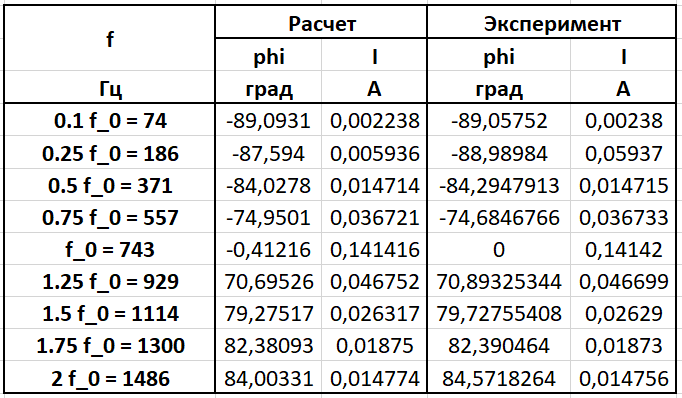
\includegraphics[width=0.7\textwidth]{8_table.png}
    \caption{Расчетная таблица для последовательного резонанса.}
    \label{fig:8_table}
\end{figure}

Теперь смоделируем параллельную RLC цепочку:
\begin{figure}[H]
    \centering
    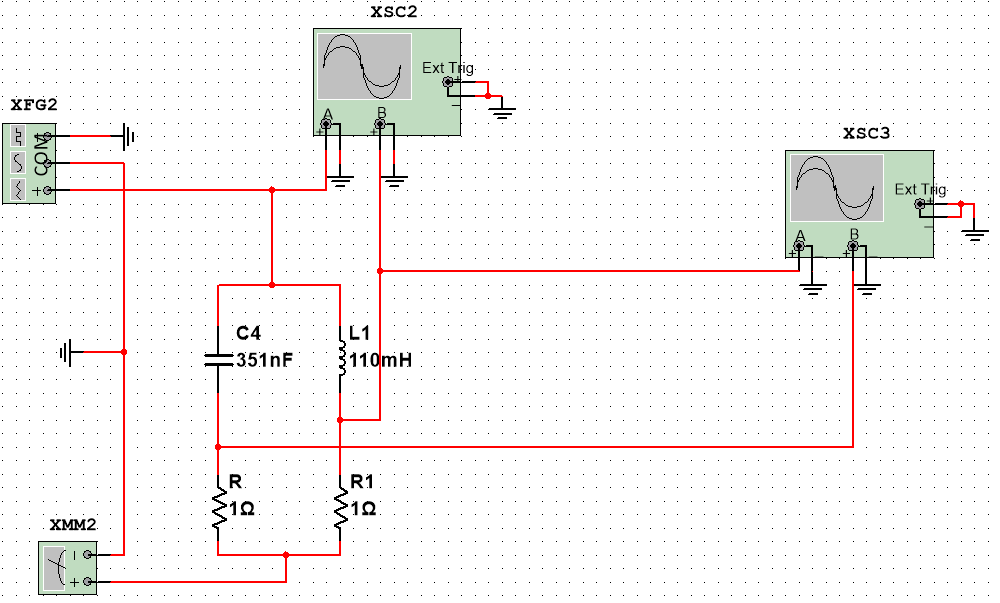
\includegraphics[width=0.7\textwidth]{9_scheme.png}
    \caption{Параллельная RLC цепочка.}
    \label{fig:9_scheme}
\end{figure}

Резонансная частота будет та же:
\[  
    f_0 = \frac{1}{2 \pi \sqrt(LC)} = 743 \ Hz
\]

Теперь установим вычисленную резонансную частоту на генераторе напряжения:
\begin{figure}[H]
    \centering
    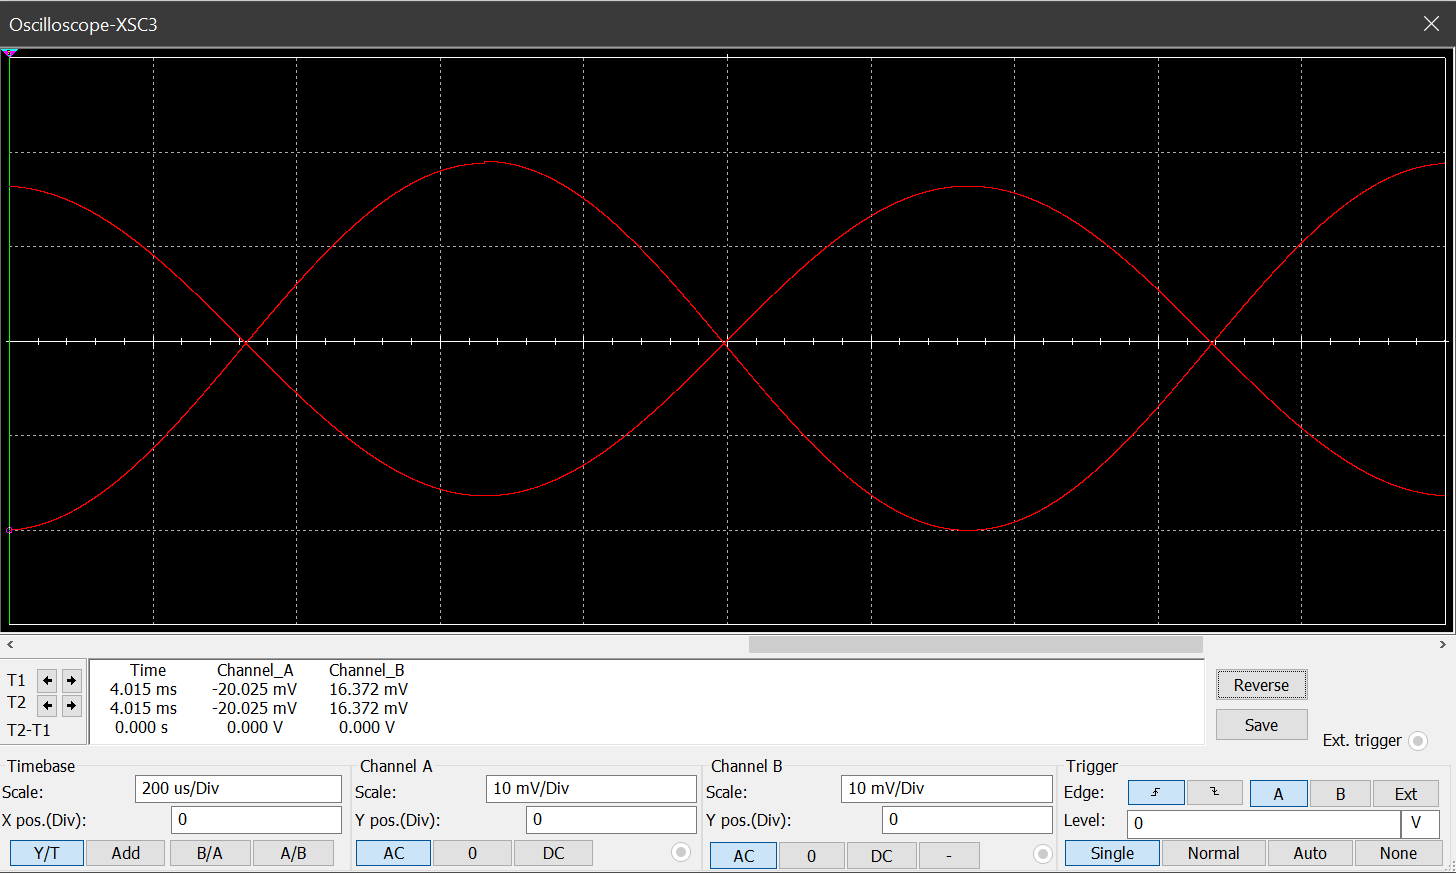
\includegraphics[width=\textwidth]{9_osc_plot.png}
    \caption{Осциллограмма при параллельном резонансе.}
    \label{fig:9_osc_plot}
\end{figure}
Можем наблюдать, что точки в ветвях равны по модулю и противоположны по фазе. \\
\ \\
Заполним следующую таблицу значениями входного тока $I$ и углами сдвига фаз $\phi$ между напряжением и током:
\begin{figure}[H]
    \centering
    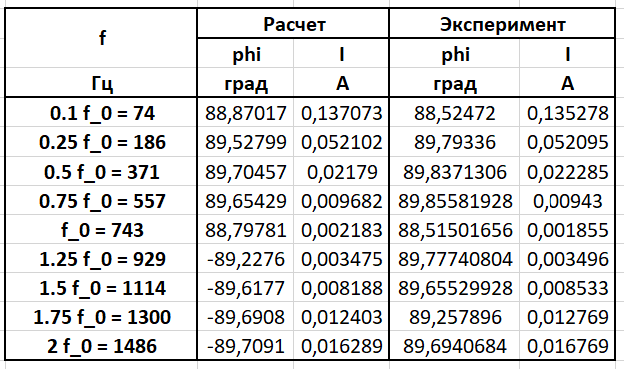
\includegraphics[width=0.7\textwidth]{9_table.png}
    \caption{Расчетная таблица для параллельного резонанса.}
    \label{fig:9_table}
\end{figure}

Экспериментальное смещение не совпало с расчетным (после точки резонансной частоты экспериментальное смещение должно было иметь противоположный знак, однако этого не наблюдалось). \\
Это произошло из-за того, что осциллограф XSC1 подключен после индуктивности, а в расчетах мы учитываем целую цепочку.

\subsubsection*{Выводы}
В ходе первой части работы были рассмотрены двухполюсники в цепи синусоидального тока. Были вычислены действующие значения тока и разность фаз входного напряжения и тока при наличии в цепи резистора, конденсатора и/или катушки индуктивности. Полученные значения схожи с расчетными значениями. \\
\ \\
В ходе выполнения второй части данной работы был рассмотрен RLC-контур в диапазоне частот, содержащем частоту, соответствующую состоянию резонанса напряжений. Были получены действующие значения тока, напряжения на резисторе, на конденсаторе и на катушке индуктивности, значения разности фаз входного напряжения и тока, для которых построенные
соответствующие зависимости от частоты колебаний напряжения в цепи. \\
Было рассмотрено два типа: параллельная и последовательная RLC-цепочка и, соответственно, два типа резонанса. \\
Все полученные данные имеют небольшое отличие с расчётными значениями, что свидетельствует о верности выполнения данной части работы.

\end{document}